\documentclass[11pt, a4paper]{article}
\usepackage{polski}
\usepackage[utf8]{inputenc}
\usepackage{graphicx}
\usepackage{amsmath}
\usepackage{float}
\usepackage{multirow}
\usepackage{afterpage}
\usepackage{longtable}
\usepackage{makecell}
\usepackage{hyperref}
\usepackage{listings}
\usepackage[margin=1in]{geometry}
\usepackage{fancyhdr}
\usepackage{adjustbox}

\title{Metody głębokiego uczenia \\
Konwolucyjne sieci neuronowe -- raport}
\author{Jadwiga Słowik}

\begin{document}
\maketitle
\section{Cel zadania}
Celem zadania jest implementacja konwolucyjnej sieci neuronowej (\textit{CNN}) klasyfikującej obrazki
ze~zbioru \textit{CIFAR-10} z~jak~największą wartością \textit{accuracy} na~zbiorze testowym.

\section{Opis zbioru danych}
\textit{CIFAR-10} (\textit{Canadian Institute For Advanced Research}) to~zbiór kolorowych obrazków o~wymiarach $32 \times 32$ pixele. Każdy~obrazek ma przydzieloną dokładnie jedną z~$10$-ciu następujących klas: samolot, samochód (\textit{ang. automobile}), ptak, kot, jeleń, pies, żaba, koń, statek, ciężarówka. Warto zaznaczyć, że~podane klasy są wykluczające.

Zbiór \textit{CIFAR-10} został podzielony na~następujące podzbiory:
\begin{enumerate}
    \item Zbiór treningowy -- $50\:000$ obrazków \\
    Składa~się z~pięciu równolicznych podzbiorów (\textit{batchy}) obrazków ułożonych w~losowej kolejności. To~znaczy, że~w~obrębie danego \textit{batcha} liczności obrazków zgrupowanych po~klasie nie~muszą być takie same.
    Aczkolwiek, sumarycznie, zbióry dla~każdej z~klas są równoliczne, tzn. jest tyle samo obrazków kotów, samochodów, itd.
    \item Zbiór testowy -- $10\:000$ obrazków \\
    Zbiór testowy jest zbalansowany, tzn. jest równomierny rozkład klas -- po~$1\:000$ wystąpień każdej klasy.
\end{enumerate}

\section{Opis konwolucyjnej sieci neuronowej}
Proces uczenia konwolucyjnej sieci neuronowej (\textit{CNN}) można podzielić na~dwie główne części: 
\begin{enumerate}
    \item Wykrywanie charakterystycznych cech obrazka
    \item Klasyfikacja
\end{enumerate}
Wykrywanie charakterystycznych cech obrazka można podzielić na~etap ,,konwolucji'' (\textit{ang. Convolution}), wprowadzenie nieliniowości (\textit{ReLU}) oraz~warstwę \textit{Pooling}.

Klasyfikacja odbywa~się na~podstawie wykrytych (przez~poprzedni etap) cech, które~są analizowane przy~pomocy sieci \textit{MLP}.

Poniżej znajduje~się szczegółowy opis każdego z~wyżej wymienionych etapów:
\begin{enumerate}
    \item \textit{Convolution} \\
    Celem operacji \textit{Convolution} jest wykrycie pewnych cech z~danego obiektu/obrazka. Owa~procedura polega na~,,przykładaniu'' konkretnego filtra (macierzy, \textit{ang. filter, kernel, feature detector}) do~macierzy z~pikselami (obrazka) i~wykonywaniu operacji mnożenia element po~elemencie (\textit{ang. element-wise}). Po~wykonaniu owej operacji mnożenia, wynikowe elementy są sumowane i~wynik (jedna liczba) jest zapisywany w~komórce nowej macierzy. W~trakcie operacji \textit{Convolution} przesuwamy ów~filtr o~wybraną liczbę elementów (parametr \textit{stride}).
    
    Możemy mieć wiele filtrów (określa~to parametr dt. głębokości (\textit{ang. depth})). Korzyścią, jaką~osiągamy dzięki~zastosowaniu większej liczby filtrów, jest możliwość ,,równoległego'' wykrywania różnych  cech obrazka np.~krawędzie poziome, pionowe, itp.
    
    Ostatecznie otrzymujemy macierz wynikową (bądź~kilka macierzy), którą~przekazujemy do~następnego etapu.
    
    \item Wprowadzenie nieliniowości \\
Na~elementach wynikowej macierzy wykonujemy wybraną funkcję nieliniową. Zwykle w~tym przypadku stosuje~się funkcję \textit{ReLU}. Uważa~się, że~działa ona znacznie lepiej niż~inne funkcje takie jak~na~przykład \textit{sigmoid} lub~\textit{tanh}.

\item \textit{Pooling} (\textit{subsampling}, \textit{downsampling}) \\
Macierze poddaje~się operacji \textit{Pooling}, której~celem jest redukcja wymiarowości macierzy otrzymanych w~poprzednim etapie przy~jednoczesnym zachowaniu istotnych cech potrzebnych w~procesie klasyfikacji.

Owa~operacja polega na~wykonywaniu wybranej funkcji (takiej jak np. maksimum, średnia, suma) na~rozłącznych grupach sąsiadujących pikseli. W~rezultacie otrzymujemy macierz, której~elementami są wyniki zastosowania wspomnianej funkcji dla~kolejnych grup sąsiadujących elementów.

Uważa~się, że~dzięki operacji \textit{Pooling} zmniejszamy prawdopodobieństwo przeuczenia i~sprawiamy, że~sieć jest mniej wrażliwa na~małe transformacje obrazka.

\item Przetwarzanie w~sieci gęstej (\textit{ang. fully connected}) \\
Ta~warstwa jest zwykłą siecią neuronową \textit{MLP}. Celem tego etapu jest klasyfikacja wynikowego (z~poprzedniego etapu) zbioru cech.

\end{enumerate}

Zbudowana przez~nas sieć \textit{CNN} może~się składać z~wielu warstw konwolucji, nieliniowości oraz~\textit{Poolingu}, które~są ze~sobą przeplatane. Dzięki~posiadaniu wielu warstw, sieć neuronowa może~lepiej uczyć~się cech, należących do~różnych klas abstrakcji. Mianowicie, pierwsze warstwy konwolucji mogą wykrywać jedynie konkretne krawędzie, podczas~gdy kolejne mogą wyspecjalizować~się w~znajdowaniu bardziej złożonych obiektów takich jak~np.uszy.

Proces uczenia polega na~znalezieniu odpowiednich współczynników filtrów i~wag sieci. Dlatego też, na~początku inicjalizujemy wagi sieci \textit{MLP} oraz~wagi filtrów losowymi wartościami.
Następnie, bierzemy~obrazek (bądź zwykle cały \textit{batch}) ze~zbioru uczącego jako~\textit{input} i~wykonujemy \textit{feed forward} przechodząc przez~wyżej wymienione etapy.
Ostatecznie, obliczamy wartość funkcji kosztu i~wykonujemy propagację wsteczną.

\section{Opis rozwiązania}
Konwolucyjne sieci neuronowe rozwiązujące problem z~różną skutecznością zostały zaimplementowane przy~użyciu biblioteki \textit{Keras} w~języku \textit{Python}. Kod zamieszczony w~\textit{jupyter-notebooku} został wykonany na~platformie \textit{Google Colab}. 

Dane dotyczące najlepszych rezultatów (tzn. modele osiągające najwyższe \textit{accuracy}) zostały zapisane w~plikach \textit{JSON} wraz~z~informacją o~procesie uczenia
i~predykcji oraz~kilka z~nich została również poddana serializacji do~plików binarnych (przy~pomocy operacji \textit{pickle} pochodzącej z~języka \textit{Python}).
Zapisane modele (i~wyniki) znajdują~się w~paczce \texttt{models\_data.zip}. Natomiast, wykorzystane kody w~niniejszej pracy są w~\textit{jupyter-notebookach} o~nazwach:
\begin{itemize}
 \item \texttt{report\_first\_models.ipynb} -- początkowe próby konstrukcji modelu sieci \textit{CNN}
 \item \texttt{report\_second.ipynb} -- zaimplementowany generator testów i~wywołania bardziej zaawansowanych modeli, których~wyniki zostały
zapisane w~plikach znajdujących~się w~paczce z~modelami
\item \texttt{report\_start\_and\_results\_analysis.ipynb} -- początkowe próby pracy z~danymi, a~później -- analiza wyników zapisanych w~paczce \texttt{models\_data.zip}
\end{itemize}

Niestety, nie~wszystkie wyniki wykonanych testów udało mi~się zamieścić w~notatnikach. Spowodowane to~zostało przez~następujące okoliczności:
\begin{enumerate}
    \item część wykonywanych testów została niespodziewanie przerwana przez~\textit{Google Colab}, pomimo~tego, że~czas ,,bezczynności notatnika'' był znacznie mniejszy niż~dwie godziny 
    \item niektóre testy po~dostatecznie dużej liczbie epok sama przerywałam i~uruchamiałam ze~zmienionymi parametrami, gdy~zauważyłam, że~sieć dalej nie~uczyła~się dostatecznie dobrze
\end{enumerate}

Jednakże, wnioski pochodzące z~wykonania ,,niepełnych'' procesów uczenia również zostały zawarte w~niniejszym raporcie.

\subsection{Zastosowane podejście}
Z~danego zbioru uczącego został klasycznie wydzielony zbiór walidacyjny, który~stanowił pierwsze $10\%$ pierwotnego zbioru.

Poniżej zostanie opisana moja droga do~ostatecznego rozwiązania: \textit{accuracy} równe $81,91\%$ (\texttt{model7.json}).

\subsubsection{Wybór optymalizatora}
Na~początku została wykonana seria eksperymentów mająca na~celu wybranie najlepszego hiperparametru dotyczącego optymalizatora. Testowane były następujące optymalizatory:
\begin{itemize}
    \item \textit{SGD}
    \item \textit{RMSprop}
    \item \textit{Adagrad}
    \item \textit{Adam}
\end{itemize}

Zdecydowanie najlepsze wyniki osiągał optymalizator \textit{SGD}: dla~danej sieci z~kilkoma warstwami konwolucji i~$20$ epokami osiągał \textit{accuracy} $67\%$, podczas gdy~pozostałe optymalizatory dawały bardzo mierne wyniki: \textit{accuracy} na~poziomie $10$-$20\%$.

\subsubsection{Wybór liczby warstw w \textit{MLP}}
Po~wykonaniu serii testów (dla~okołu $10$ epok) doszłam do~wniosku, że~zastosowanie więcej niż~jednej/dwóch warstw ukrytych pogarsza wyniki klasyfikacji. Wobec~tego, ten hiperparametr ustawiłam na~wartość równą $2$. W~każdej warstwie ukrytej znajdowało~się $128$ neuronów z~funkcją aktywacji \textit{ReLU}.

\subsubsection{Wybór konfiguracji warstwy \textit{poolingowo}-\textit{konwolucyjnej}}
Napisałam pomocnicze funkcje do~generowania testów (kod jest zawarty w~\textit{jupyter-notebooku} \texttt{report\_second}). Przy~ich pomocy mogłam w~łatwy sposób wywoływać testy z~różnymi konfiguracjami (np.~określona liczba warstw konwolucyjnych itp.).

Wyniki tej serii testów przedstawiają~się następująco (parametr \textit{learning rate} został ustawiony na~wartość $0,01$):

\begin{table}[H]
    \centering
    \begin{tabular}{|c|c|c|c|c|}
    \hline
      \textbf{id} & \textbf{conv\_num} & \textbf{pooling\_iter} & \textbf{epochs} & \textbf{accuracy} \\
        \hline
    $1$ &    $1 + 3$ & $1$ & $5$ & $63\%$ \\
        \hline
    $2$ &    $1 + 10$ & $1$ & $5$ & $61\%$ \\
        \hline
    $3$ &    $1 + 30$ & $1$ & $5$ & $47\%$ \\
        \hline
    $4$ &    $1 + 3$ & $4$ & $5$ & $62\%$  \\
        \hline
    $5$ &    $1 + 8$ & $4$ & $5$ & $17\%$ \\
    \hline
    $6$ & $1 + 3$ & $4$  & $40$ & $76\%$ \\
    \hline
    \end{tabular}
    \caption{Wyniki testów dla~różnych konfiguracji warstwy \textit{poolingowo}-\textit{konwolucyjnej}}
\end{table}

W~kolumnie \textit{conv\_num} liczba warstw konwolucji została przedstawiona przy~pomocy sumy, gdyż~pierwsza warstwa miała filtry o~wymiarach $3 \times 3$, natomiast następne warstwy miały wymiary $2 \times 2$.
Głębokość (liczba \textit{filtrów}) każdej warstwy konwolucji wynosiła $128$.

Jako że~sieci były uruchamiane na~platformie \textit{Google Colab}, gdzie~wystąpują ograniczenia czasowe związane z~wykonywanymi obliczeniami, musiałam znacząco okroić liczbę konfiguracji sieci, które~miałam zamiar testować, gdyż~niemożliwe było zostawienie dłuższych obliczeń bez~nadzoru.

Intuicyjnie, sieć o~numerze porządkowym równym $4$ zachowywała~się bardzo obiecująco przy~małej liczbie epok, dlatego~też zdecydowałam~się na~sprawdzenie jej skuteczności dla~większej liczby. Ostatecznie, postanowiłam optymalizować inne hiperparametry tej właśnie sieci.

\subsubsection{Zastosowanie metod regularyzacji}
Zastosowanie metod regularyzacji ma~na~celu wyeliminowanie zjawiska przeuczenia~się sieci (\textit{overfittingu}), czyli~zbyt dużego dopasowania~się do~danych treningowych bez~zdolności generalizacji na~inne przypadki.

Podjęłam~się zastosowania następujących metod:
\begin{itemize}
    \item \textit{Kernel regularizer} dla~wartstw \textit{fully connected} i~warstw konwolucyjnych 
    \item \textit{Dropout} (prawdopodobieństwo wygaszenia połączenia równe $0,2$) \\
    Ideą metody \textit{dropout} jest wygaszanie losowych połączeń w~sieci neuronowej. Zastosowałam \textit{dropout} dla~każdej warstwy sieci.
    \item \textit{Batch Normalization} \\
    Owa metoda poddaje normalizacji wynik (\textit{aktywację}) poprzedniej warstwy.
\end{itemize}
Wykorzystanie pierwsze metody spowodowało znaczący spadek skuteczności klasyfikacji do~rzędu $20\%$,
natomiast że~zastosowanie dwóch ostatnich metod poprawiło wynik o~kilka punktów procentowych (\textit{accuracy} rzędu \textit{79\%}).


\subsubsection{Pierwsza próba zastosowania \textit{data augmentation}}
Podjęłam pierwszą próbę zastosowania \textit{data augmentation} (przy~pomocy obiektu \textit{ImageDataGenerator} z~biblioteki \textit{Keras}) z~następującymi operacjami na~obrazkach:
\begin{itemize}
    \item \texttt{width\_shift\_range} $ = 0,1$
    \item \texttt{height\_shift\_range} $= 0,1$
    \item \texttt{shear\_range} $ = 0,2 $
    \item \texttt{zoom\_range} $ = 0,3$
    \item \texttt{horizontal\_flip} oraz~\texttt{vertical\_flip}
\end{itemize}

Zauważyłam, że~od pewnego momentu wartości \textit{accuracy} dla~zbioru walidacyjnego i~treningowego prawie nie~ulegają zmianie -- utrzymują~się w~okolicach $78\%$.
Po~wykonaniu $150$ epok, skuteczność sieci dla~danych testowych była podobna.

Podejrzewam, że~zatrzymanie skuteczności uczenia mogło być spowodowane przez~dwa następujące czynniki:
\begin{itemize}
    \item Ustawiłam zbyt dużo różnych przekształceń obrazka, w~wyniku czego generowane obrazki nie~były dostatecznie użyteczne dla~procesu uczenia sieci i~również, z~powodu dużej liczby możliwości -- niektóre (być~może bardziej przydatne transformacje) miały mniejsze prawdopodobieństwo bycia wygenerowanym
    \item Została zastosowana jedna wartość \textit{learning rate} \\
    Przypuszczam, że~w~tym przypadku zastosowanie mniejszego \textit{learning rate} dla~większych numerów epok mogłoby przynieść poprawę skuteczności klasyfikacji
\end{itemize}

\subsubsection{Wybór \textit{stałej uczenia}}
Na~początku testowałam zachowanie sieci w~przypadku, gdy~nie~zmieniałam \textit{explicite} wartości \textit{stałej uczenia}. Ustawiałam ją na~następujące wartości: $0,01$,\, $0,001$,\, $0,0005$. Zauważyłam jednak, że~przy ustawianiu mniejszej wartości sieć wolniej~się uczy i~wymaga większej liczby epok, aby~osiągnąć dobrą skuteczność.

Wobec~tego, zdecydowałam~się na~zastosowanie zmiennej wartości stałej uczenia w~zależności od~numeru epoki, która~jest aktualnie wykonywana. Mianowicie, dla~numeru epoki:
\begin{itemize}
    \item w~przedziale $[1, 30)$: \textit{learning rate} równy $0,01$
    \item w~przedziale $[30, 60)$: \textit{learning rate} równy $0,005$
    \item w~przedziale $[60, \infty)$: \textit{learning rate} równy $0,003$
\end{itemize}
Niestety, zastosowany zabieg nie~poprawił jakości klasyfikacji. Testowany był dla~$80$ epok (\texttt{model8.json}). Być~może, zwiększenie liczby epok poprawiłoby jakość \textit{accuracy}. Niestety, fizycznie nie~byłabym w~stanie wykonać obliczeń trwających ponad~parenaście godzin pracując na~platformie \textit{Google Colab}.

\subsubsection{Druga próba zastosowania \textit{data augmentation}}
Wyciągnowszy wnioski z~powyżej opisanego podejścia, postanowiłam wykonać drugą próbę.
Postanowiłam \textit{douczyć} wcześniej wytrenowany model (\texttt{model7.json} o~skuteczności ok. $82\%$) dodając \textit{data augmentation}.

Zastosowałam zmienny (w~zależności od~numeru epoki) \textit{learning rate} (liczony według~algorytmu opisanego we~wcześniejszym punkcie) oraz~ograniczyłam możliwości transformacji obrazka do~następujących parametrów:
\begin{itemize}
    \item \texttt{rotation\_range} $=30$
    \item \texttt{width\_shift\_range} i~\texttt{width\_shift\_range} równe $0,1$
    \item \texttt{horizontal\_flip} i~\texttt{vertical\_flip}
\end{itemize}
Proces uczenia został ustawiony na~$100$ epok. Niestety, \textit{Google Colab} niespodziewanie przerwał moje obliczenia w~$75$-tej epoce pomimo faktu, że~około~$10$~minut wcześniej dokonywałam modyfikacji w~\textit{jupyter-notebooku}.
Jednakże, wyniki uzystane do~$75$-tej epoki nie~wyglądają optymistycznie: od~pewnego momentu \textit{accuracy} oscyluje w~granicach $80\%$ i~sieć ma~spore trudności, aby~tę wartość przekroczyć.

\subsection{Opis ostatecznego rozwiązania}
W~niniejszym rozdziale zostanie opisane rozwiązanie dające najwyższą skuteczność.
\subsubsection{Architektura}
Sieć uzyskująca najwyższą skuteczność na~zbiorze testowym ($81,91\%$) ma~następującą architekturę:
\begin{enumerate}
    \item Jedna warstwa konwolucji o~głębokości równej $128$ i~wymiarze filtra $3 \times 3$ i~przesunięciu $1$
    \item Nieliniowość \textit{ReLU}
    \item $4$ warstwy \textit{MaxPooling} o~wymiarze $2 \times 2$ i~przesunięciu równym $2$ (operacja \textit{pooling} była wykonywana po~każdej warstwie konwolucyjnej opisanej poniżej). W~obrębie każdej warstwy:
        \begin{enumerate}
            \item Warstwa konwolucji: głębokość równa $128$, wymiar filtra $2 \times 2$ oraz~wartość przesunięcia (\textit{ang. stride}) równa $1$
            \item Nieliniowość \textit{ReLU}
            \item \textit{Dropout} z~prawdopodobieństwem $0,2$
            \item \textit{BatchNormalization}
            \item Warstwa konwolucji: głębokość równa $128$, wymiar filtra $2 \times 2$ oraz~wartość przesunięcia (\textit{ang. stride}) równa $1$
            \item Nieliniowość \textit{ReLU}
            \item \textit{Dropout} z~prawdopodobieństwem $0,2$
            \item \textit{BatchNormalization}
            \item Warstwa konwolucji: głębokość równa $128$, wymiar filtra $2 \times 2$ oraz~wartość przesunięcia (\textit{ang. stride}) równa $1$
            \item Nieliniowość \textit{ReLU}
            \item \textit{Dropout} z~prawdopodobieństwem $0,2$
            \item \textit{BatchNormalization}
        \end{enumerate}
    \item Warstwa \textit{Fully-connected} z~liczbą neuronów równą~$128$ i~funkcją aktywacji $ReLU$
    \item \textit{Dropout} równy $0,2$
    \item \textit{BatchNormalization}
    \item Warstwa \textit{Fully-connected} z~liczbą neuronów równą~$128$ i~funkcją aktywacji $ReLU$
    \item \textit{Dropout} równy $0,2$
    \item \textit{BatchNormalization}
    \item Wartstwa wyjściowa z~liczbą neuronów równą $10$ (liczba klas) i~funkcją aktywacji \textit{softmax}
\end{enumerate}

Proces uczenia powyższej sieci trwał $50$ epok i~wartość \textit{learning rate} była stała (o~wartości $0,01$).

\subsubsection{Funkcja kosztu}
Wykres funkcji kosztu obliczanej w~trakcie trenowania sieci dla~zbioru treningowego i~walidacyjnego przedstawia~się następująco:
\begin{figure}[H]
\centering
    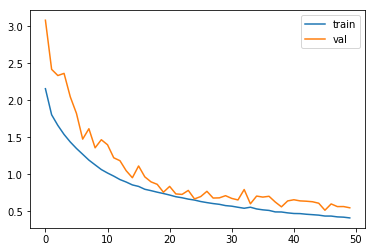
\includegraphics[scale=0.8]{funkcja_kosztu.png}
    \caption{Wykres funkcji kosztu}
\end{figure}

\subsubsection{Wykresy \textit{ROC}}
Poniżej znajdują~się wykresy \textit{ROC} dla~każdej klasy:
\begin{figure}[H]
\centering
    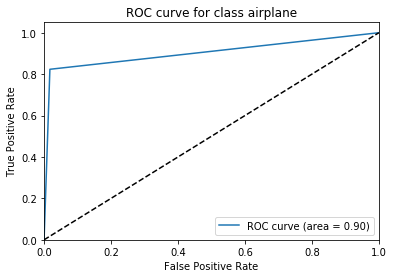
\includegraphics[scale=0.8]{roc_0.png}
    \caption{Wykres \textit{ROC} z~wartościami \textit{AUC} dla~klasy \textit{airplane}}
\end{figure}
\begin{figure}[H]
\centering
    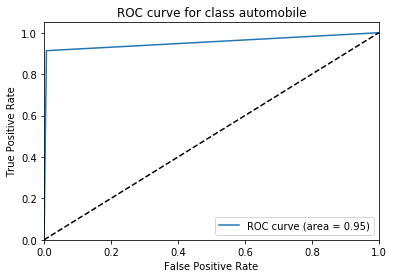
\includegraphics[scale=0.8]{roc_1.png}
    \caption{Wykres \textit{ROC} z~wartościami \textit{AUC} dla~klasy \textit{automobile}}
\end{figure}
\begin{figure}[H]
\centering
    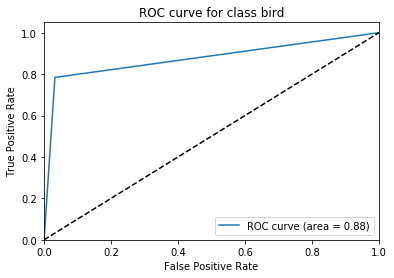
\includegraphics[scale=0.8]{roc_2.png}
    \caption{Wykres \textit{ROC} z~wartościami \textit{AUC} dla~klasy \textit{bird}}
\end{figure}
\begin{figure}[H]
\centering
    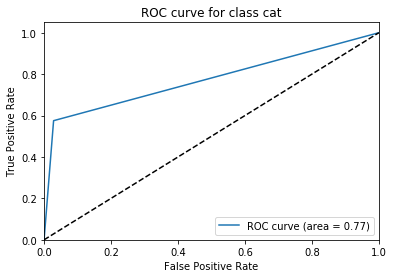
\includegraphics[scale=0.8]{roc_3.png}
    \caption{Wykres \textit{ROC} z~wartościami \textit{AUC} dla~klasy \textit{cat}}
\end{figure}
\begin{figure}[H]
\centering
    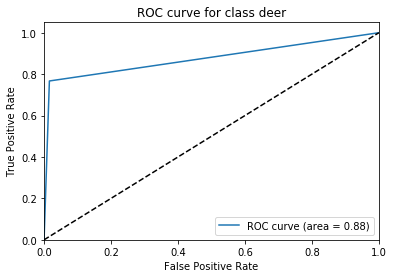
\includegraphics[scale=0.8]{roc_4.png}
    \caption{Wykres \textit{ROC} z~wartościami \textit{AUC} dla~klasy \textit{deer}}
\end{figure}
\begin{figure}[H]
\centering
    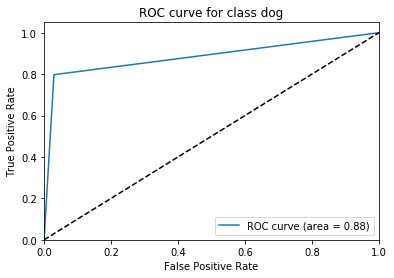
\includegraphics[scale=0.8]{roc_5.png}
    \caption{Wykres \textit{ROC} z~wartościami \textit{AUC} dla~klasy \textit{dog}}
\end{figure}
\begin{figure}[H]
\centering
    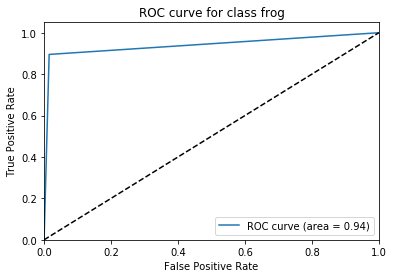
\includegraphics[scale=0.8]{roc_6.png}
    \caption{Wykres \textit{ROC} z~wartościami \textit{AUC} dla~klasy \textit{frog}}
\end{figure}
\begin{figure}[H]
\centering
    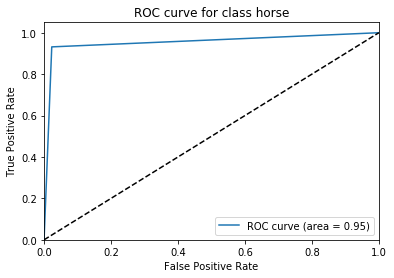
\includegraphics[scale=0.8]{roc_7.png}
    \caption{Wykres \textit{ROC} z~wartościami \textit{AUC} dla~klasy \textit{horse}}
\end{figure}
\begin{figure}[H]
\centering
    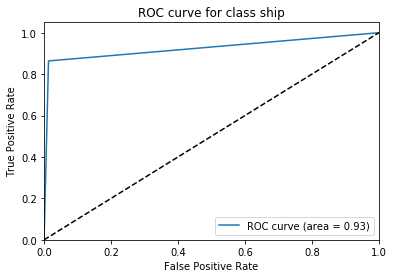
\includegraphics[scale=0.8]{roc_8.png}
    \caption{Wykres \textit{ROC} z~wartościami \textit{AUC} dla~klasy \textit{ship}}
\end{figure}
\begin{figure}[H]
\centering
    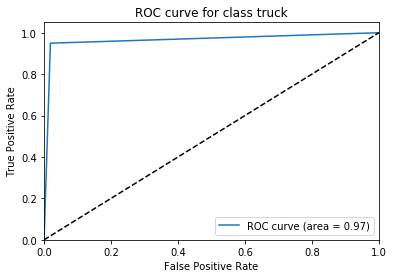
\includegraphics[scale=0.8]{roc_9.png}
    \caption{Wykres \textit{ROC} z~wartościami \textit{AUC} dla~klasy \textit{truck}}
\end{figure}

Na~podstawie powyższych wykresów można stwierdzić, że~zdecydowanie najgorszy wynik osiąga klasyfikacja kotów.
Lista wszystkich źle sklasyfikowanych obrazków znajduje~się w~pliku \textit{jupyter-notebooka} \texttt{report\_start\_and\_tests\_analysis}.

Poniżej znajduje~się zbiorczy wykres \textit{ROC}.
\begin{figure}[H]
\centering
    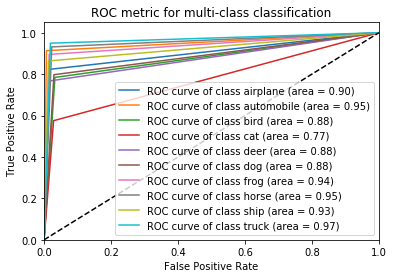
\includegraphics[scale=0.8]{roc.png}
    \caption{Wykres \textit{ROC} z~wartościami \textit{AUC} dla~każdej klasy}
\end{figure}


\subsubsection{Macierz pomyłek}
Macierz pomyłek (\textit{ang. confusion matrix}) przedstawia~się następująco
\begin{figure}[H]
 \centering
  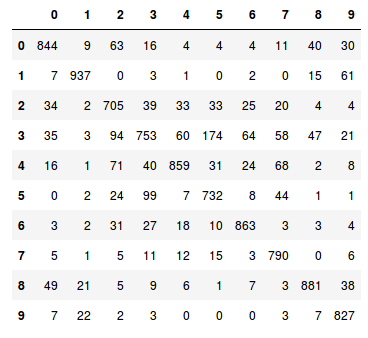
\includegraphics[scale=1]{confusion_matrix.png}
  \caption{Macierz pomyłek}
\end{figure}
Wiersze macierzy oznaczają wartość oczekiwaną, natomiast kolumny -- wartość przewidzianą przez~model.
Z~powyższej macierzy można wywnioskować, że~bardzo dużo pomyłek występuje przy~próbie klasyfikacji obrazka z~kotem.


\subsection{Pomysły na ulepszenie rozwiązania}
Gdybym miała więcej czasu i~lepsze warunki obliczeniowe, to~spróbowałabym dodać do~powyższej architektury \textit{data augmentation}, ze~zmienną (malejącą wraz ze~wzrostem numeru epoki) wartością \textit{learning rate} oraz~znacznie większą liczbą epok (ponad~$200$).

Również, ciekawym pomysłem byłoby wykorzystanie pretrenowanej sieci i~zastosowanie tzw.~\textit{transfer learning}.

Ponadto, następnym razem, aby~zabezpieczyć~się przez~niespodziewanym zamknięciem sesji przez~\textit{Google Colab}, mogłabym zapisywać model, co~pewną, wybraną liczbę epok.
\end{document}
